%!TEX root = ../larxxia.tex

\section{Linear combinations span sets}
\label{sec:lcss}
\secttoc

\begin{comment}
\pooliv{\S2.3} \layiv{\S1.3} \holti{\S2.1--2} \nakos{\S2.3}
\end{comment}



A common feature in the solution to linear equations is the  appearance of combinations of several vectors.
For example, the general solution to Example~\ref{eg:homosysiv}  is 
\begin{eqnarray*}
\xv&=&(-2s-\tfrac{15}7t,s,\tfrac97t,t) 
\\&=&\underbrace{s(-2,1,0,0)+t(-\tfrac{15}7,0,\tfrac97,1)}_{\text{linear combination}}.
\end{eqnarray*}
The general solution to Example~\ref{eg:rrefi} is
\begin{eqnarray*}
\xv&=&(-2-s+2t,s,5-4t,t)
\\&=&\underbrace{1\cdot(-2,0,5,0)+s(-1,1,0,0)+t(2,0,-4,1)}_{\text{linear combination}}.
\end{eqnarray*}
Such so-called \idx{linear combination}s occur in many other contexts.
Recall the standard unit vectors in~\(\RR^3\) are \(\ev_1=(1,0,0)\), \(\ev_2=(0,1,0)\) and \(\ev_3=(0,0,1)\) (Definition~\ref{def:stuniv}): any other vector in~\(\RR^3\) may be written as
\begin{eqnarray*}
\xv&=&(x_1,x_2,x_3)
\\&=&x_1(1,0,0)+x_2(0,1,0)+x_3(0,0,1)
\\&=&\underbrace{x_1\ev_1+x_2\ev_2+x_3\ev_3}_{\text{linear combination}}.
\end{eqnarray*}
The wide-spread appearance of such `linear combinations' calls for the following definition.

\begin{definition} \label{def:lincom}
A vector~\vv\ is a \bfidx{linear combination} of vectors \hlist\vv k\ if there are scalars \hlist ck\ (called the \bfidx{coefficient}s) such that \(\vv=\lincomb c\vv k\)\,.
\end{definition}


\begin{example} \label{eg:}
Estimate roughly each of the blue vectors as a \idx{linear combination} of the given red vectors in the following graphs (estimate coefficients to say 10\%~error).
\begin{parts}
\item 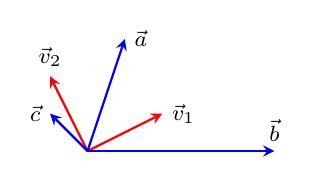
\begin{tikzpicture} 
\begin{axis}[footnotesize,font=\footnotesize%,domain=-1.5:1.5
    ,axis equal image, axis lines=none    ] 
    \addplot[red,thick,quiver={u=2,v=1},-stealth] coordinates {(0,0)};
    \node[right] at (axis cs:2,1) {$\vec v_1$};
    \addplot[red,thick,quiver={u=-1,v=2},-stealth] coordinates {(0,0)};
    \node[above] at (axis cs:-1,2) {$\vec v_2$};
    \addplot[blue,thick,quiver={u=1,v=3},-stealth] coordinates {(0,0)};
    \node[right] at (axis cs:1,3) {$\vec a$};
    \addplot[blue,thick,quiver={u=5,v=0},-stealth] coordinates {(0,0)};
    \node[above] at (axis cs:5,0) {$\vec b$};
    \addplot[blue,thick,quiver={u=-1,v=1},-stealth] coordinates {(0,0)};
    \node[left] at (axis cs:-1,1) {$\vec c$};
\end{axis}
\end{tikzpicture}
\begin{solution} 
By visualising various combinations: 
vector \(\av\approx -1\vv_1+4\vv_2\)\,;
vector \(\bv\approx 2\vv_1-2\vv_2\)\,;
vector \(\cv\approx -1\vv_1+2\vv_2\)\,. 
\end{solution}



\item 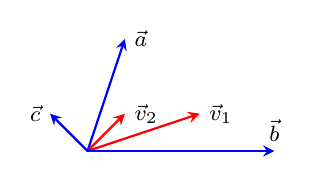
\begin{tikzpicture} 
\begin{axis}[footnotesize,font=\footnotesize%,domain=-1.5:1.5
    ,axis equal image, axis lines=none    ] 
    \addplot[red,thick,quiver={u=3,v=1},-stealth] coordinates {(0,0)};
    \node[right] at (axis cs:3,1) {$\vec v_1$};
    \addplot[red,thick,quiver={u=1,v=1},-stealth] coordinates {(0,0)};
    \node[right] at (axis cs:1,1) {$\vec v_2$};
    \addplot[blue,thick,quiver={u=1,v=3},-stealth] coordinates {(0,0)};
    \node[right] at (axis cs:1,3) {$\vec a$};
    \addplot[blue,thick,quiver={u=5,v=0},-stealth] coordinates {(0,0)};
    \node[above] at (axis cs:5,0) {$\vec b$};
    \addplot[blue,thick,quiver={u=-1,v=1},-stealth] coordinates {(0,0)};
    \node[left] at (axis cs:-1,1) {$\vec c$};
\end{axis}
\end{tikzpicture}
\begin{solution} 
By visualising various combinations: 
vector \(\av\approx -1\vv_1+4\vv_2\)\,;
vector \(\bv\approx 2\vv_1-2\vv_2\)\,;
vector \(\cv\approx -1\vv_1+2\vv_2\)\,. 
\end{solution}

\end{parts}
%\begin{solution} 
%\begin{enumerate}
%\item By visualising various combinations: 
%vector \(\av\approx \vv_1+\vv_2=1\vv_1+1\vv_2\)\,;
%vector \(\bv\approx 2\vv_1-\vv_2=2\vv_1+(-1)\vv_2\)\,;
%vector \(\cv\approx -0.2\vv_1+0.6\vv_2\)\,.
%
%\item By visualising various combinations: 
%vector \(\av\approx -1\vv_1+4\vv_2\)\,;
%vector \(\bv\approx 2\vv_1-2\vv_2\)\,;
%vector \(\cv\approx -1\vv_1+2\vv_2\)\,.
%
%\end{enumerate}
%\end{solution}
\end{example}



\begin{example} \label{eg:lcs}
\index{parametric equation}Parametric descriptions of lines and planes  involve \idx{linear combination}s (Sections~\ref{sec:asv}--\ref{sec:dpdal}).
\begin{enumerate}
\item 
For each value of~\(t\), \((3,4)+t(-1,2)\) is a linear combination of the two vectors \((3,4)\) and~\((-1,2)\).  
Over all values of parameter~\(t\) it describes the line illustrated in the margin.
(The line is alternatively described as \(2x+y=10\)\,.)
\marginpar{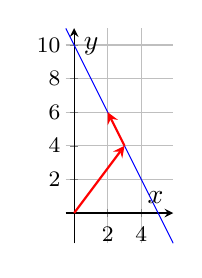
\begin{tikzpicture}[]
\begin{axis}[footnotesize
    , axis equal image, axis lines=middle,
    , xlabel={$x$},ylabel={$y$},  grid, domain=-0.5:5.9
    ]
    \addplot[blue]{10-2*x} ;
    \addplot[red,quiver={u=3,v=4},-stealth,thick] coordinates {(0,0)};
    \addplot[red,quiver={u=-1,v=2},-stealth,thick] coordinates {(3,4)};
\end{axis}
\end{tikzpicture}}

\item For each value of \(s\) and~\(t\), \(2(1,0,1)+s(-1,-\frac12,\frac12)+t(1,-1,0)\) is a linear combination of the three vectors \((1,0,1)\), \((-1,-\frac12,\frac12)\) and~\((1,-1,0)\).
Over all values of the parameters~\(s\) and~\(t\) it describes the plane illustrated below.
(Alternatively the plane could be described as \(x+y+3z=8\)).
%\marginpar{%
\begin{center}
\foreach \q in {37,40} {\begin{tikzpicture}
\begin{axis}[footnotesize,view={\q}{30}
    , xlabel={$x$},ylabel={$y$},zlabel={$z$},label shift={-1.5ex}
    , grid, domain=0:4
    ]
    \addplot3[surf,shader=interp,opacity=0.3,samples=2,y domain=-2:1] {(-x-y+8)/3};
    \addplot3[red,quiver={u=1,v=0,w=1},-stealth,thick] coordinates {(0,0,0)(1,0,1)};
    \addplot3[red,quiver={u=-1,v=-1/2,w=1/2},-stealth,thick] coordinates {(2,0,2)};
    \addplot3[red,quiver={u=1,v=-1,w=0},-stealth,thick] coordinates {(2,0,2)};
\end{axis}
\end{tikzpicture}}
\end{center}


\item 
\(t(-1,2,0)+t^2(0,2,1)\)
is a linear combination of the two vectors \((-1,2,0)\) and~\((0,2,1)\) as the vectors are multiplied by scalars and then added.  
That a coefficient is a nonlinear function of some parameter is irrelevant to the property of linear combination.
This expression is the parametric description of a parabola in~\(\RR^3\), as illustrated below, and very soon we will be able to say it is a parabola in the plane spanned by \((-1,2,0)\) and~\((0,2,1)\).
%\marginpar{%
\begin{center}
\foreach \q in {37,40} {\begin{tikzpicture}
\begin{axis}[footnotesize,view={\q}{30}
    , grid, domain=-1:1]
    \addplot3[blue,samples y=0,thick]({-x},{2*x+2*x^2},{x^2});
    \addplot3[surf,shader=interp,opacity=0.3,samples=2,y domain=-0.5:4] {x+y/2};
    \addplot3[red,quiver={u=-1,v=2,w=0},-stealth,thick] coordinates {(0,0,0)};
    \addplot3[red,quiver={u=0,v=2,w=1},-stealth,thick] coordinates {(0,0,0)};
\end{axis}
\end{tikzpicture}}
\end{center}

\end{enumerate}
\end{example}



\begin{example} \label{eg:lcmatvec}
The \idx{matrix-vector form} \(A\xv=\bv\) of a system of linear equations involves a \idx{linear combination} on the left-hand side.
Recall from Definition~\ref{def:matvecsys} that \(A\xv=\bv\) is our abstract abbreviation for the system of \(m\)~equations
\begin{eqnarray*}
&&a_{11}x_1+a_{12}x_2+\cdots+a_{1n}x_n=b_1\,,
\\&&a_{21}x_1+a_{22}x_2+\cdots+a_{2n}x_n=b_2\,,
\\&&\quad\vdots
\\&&a_{m1}x_1+a_{m2}x_2+\cdots+a_{mn}x_n=b_m\,.
\end{eqnarray*}
Form both sides into a vector so that
\begin{equation*}
\begin{bmatrix} 
a_{11}x_1+a_{12}x_2+\cdots+a_{1n}x_n
\\a_{21}x_1+a_{22}x_2+\cdots+a_{2n}x_n
\\\vdots
\\a_{m1}x_1+a_{m2}x_2+\cdots+a_{mn}x_n
\end{bmatrix}
=\begin{bmatrix}b_1\\b_2\\\vdots\\b_m \end{bmatrix}.
\end{equation*}
Then use addition and scalar multiplication of vectors (Definition~\ref{def:vecops}) to rewrite the left-hand side vector as
\begin{equation*}
\begin{bmatrix} a_{11}\\a_{21}\\\vdots\\a_{m1}\end{bmatrix}x_1
+\begin{bmatrix} a_{12}\\a_{22}\\\vdots\\a_{m2}\end{bmatrix}x_2
+\cdots
+\begin{bmatrix} a_{1n}\\a_{2n}\\\vdots\\a_{mn}\end{bmatrix}x_n
=\begin{bmatrix} b_1\\b_2\\\vdots\\b_m \end{bmatrix}.
\end{equation*}
This left-hand side is a linear combination of the columns of matrix~\(A\): define from the columns of~\(A\) the \(n\)~vectors, \(\av_1=(a_{11},a_{21},\ldots,a_{m1})\), \(\av_2=(a_{12},a_{22},\ldots,a_{m2})\), \ldots, \(\av_n=(a_{1n},a_{2n},\ldots,a_{mn})\), then the left-hand side is a linear combination of these vectors, with the coefficients of the linear combination being \hlist xn.
\end{example}

\begin{aside}
Be aware of a subtle twist going on here: this theorem turns a question about the existence of \(n\)~variable solution~\xv, into a question about vectors with \(m\)~components; and vice-versa.
\end{aside}
\begin{theorem} \label{thm:conlincom} 
A system of \idx{linear equation}s \(A\xv=\bv\) is \idx{consistent} (Procedure~\ref{pro:gje}) if and only if the right-hand side vector~\bv\ is a \idx{linear combination} of the columns of~\(A\).
\end{theorem}

\begin{proof} 
Example~\ref{eg:lcmatvec} establishes that if a solution~\xv\ exists, then \bv~is a linear combination of the columns.
Conversely, if \bv~is a linear combination of the columns, then a solution~\xv\ exists with components of~\xv\ set to the coefficients in the linear combination.
\end{proof}


\begin{example} \label{eg:}
This first example considers the simplest case when the matrix has only one column, and so any linear combination is only a scalar multiple of that column.
Compare the consistency of the equations with the right-hand side being a linear combination of the column of the matrix.
\begin{enumerate}
\item \(\begin{bmatrix} -1\\2 \end{bmatrix}x
=\begin{bmatrix} -2\\4 \end{bmatrix}\).
\begin{solution} 
The system is consistent because \(x=2\) is a solution (Procedure~\ref{pro:gje}).
Also, the right-hand side \(\bv=(-2,4)\) is the linear combination \(2(-1,2)\) of the column of the matrix.
\end{solution}

\item \(\begin{bmatrix} -1\\2 \end{bmatrix}x
=\begin{bmatrix} 2\\3 \end{bmatrix}\).
\begin{solution} 
The system is inconsistent as the first equation requires \(x=-2\) whereas the second requires \(x=\tfrac32\) and these cannot hold simultaneously (Procedure~\ref{pro:gje}).
Also, there is no multiple of \((-1,2)\) that gives the right-hand side \(\bv=(2,3)\) so the right-hand side cannot be a linear combination of the column of the matrix---as illustrated in the margin.
\marginpar{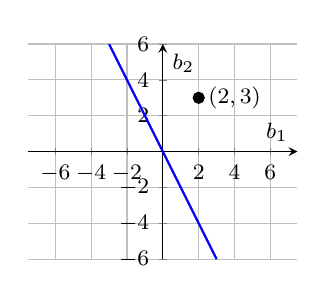
\begin{tikzpicture} 
\begin{axis}[footnotesize,font=\footnotesize
    ,axis equal, axis lines=middle, grid,domain=-3:3
    ,xlabel={$b_1$}, ylabel={$b_2$} ] 
    \addplot[blue,thick] {-2*x};
    \addplot[black, mark=*] coordinates {(2,3)} node[right] {\((2,3)\)};
\end{axis}
\end{tikzpicture}}
\end{solution}

\item \(\begin{bmatrix} 1\\a \end{bmatrix}x
=\begin{bmatrix} 3\\-6 \end{bmatrix}\) depending upon parameter~\(a\).
\begin{solution} 
The first equation requires \(x=3\) whereas the second equation requires \(ax=-6\); that is, \(a\cdot3=-6\)\,, that is, \(a=-2\)\,.
Thus it is only for \(a=-2\) that the system is consistent;
for \(a\neq-2\) the system is inconsistent.
Also, plotted in the margin are vectors \((1,a)\) for various~\(a\).
It is only for \(a=-2\) that the vector is aligned towards the given \((3,-6)\).
Hence it is only for \(a=-2\) that a linear combination of~\((1,a)\) can give the required~\((3,-6)\).
\marginpar{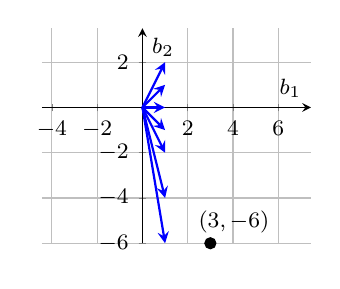
\begin{tikzpicture} 
\begin{axis}[footnotesize,font=\footnotesize
    ,axis equal, axis lines=middle, grid,domain=-1:3
    ,xlabel={$b_1$}, ylabel={$b_2$}, ymax=3.5 ] 
    \foreach \a in {2,1,0,-1,-2,-4,-6} {
    \addplot[blue,thick,-stealth,quiver={u=1,v=\a}] coordinates {(0,0)};
    };
    \addplot[black, mark=*] coordinates {(3,-6)}
     node[above] {\qquad\((3,-6)\)};
\end{axis}
\end{tikzpicture}}
\end{solution}

\end{enumerate}
\end{example}



In the examples of linear combination, the coefficients mostly involve a variable parameter or unknown.
Consequently, mostly we are interested in the range of possibilities encompassed by a given set of vectors.


\begin{definition} \label{def:span} 
Let a set of vectors in~\(\RR^n\) be  \(S=\{\hlist\vv k\}\), then the set of all \idx{linear combination}s of \hlist\vv k\ is called the \bfidx{span} of \hlist\vv k, and is denoted by \(\Span\{\hlist\vv k\}\) or \(\Span S\)\,.%
\footnote{In the degenerate case of the set~\(S\) being the empty set, we take its span to be just the zero vector; that is, by convention \(\Span\{\}=\{\ov\}\).  But we rarely need this degenerate case.}
%If \(\Span S=\RR^n\), then \(S\) is called a \bfidx{spanning set} for~\(\RR^n\).
\end{definition}


\begin{example} \label{eg:span}
\begin{enumerate}
\item Let the set \(S=\{(-1,2)\}\) with just one vector.  Then \(\Span S=\Span\{(-1,2)\}\) is the set of all vectors encompassed by the form \(t(-1,2)\): from the parametric equation of a line (Definition~\ref{def:parlin}), \(\Span S\) is all vectors in the line \(y=-2x\) as shown in the margin.
\marginpar{%
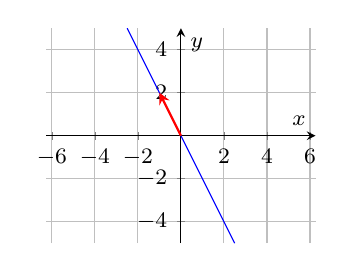
\begin{tikzpicture}[]
\begin{axis}[footnotesize,font=\footnotesize
    , axis equal, axis lines=middle,
    , xlabel={$x$},ylabel={$y$},  grid, domain=-2.5:2.5
    ]
    \addplot[blue]{-2*x} ;
    \addplot[red,quiver={u=-1,v=2},-stealth,thick] coordinates {(0,0)};
\end{axis}
\end{tikzpicture}
}

\item With two vectors in the set, \(\Span\{(-1,2),(3,4)\}=\RR^2\) is the entire 2D plane.
To see this, recall that any point in the span must be of the form \(s(-1,2)+t(3,4)\).
Given any vector \((x_1,x_2)\) in~\(\RR^2\) we choose \(s=(-4x_1+3x_2)/10\) and \(t=(2x_1+x_2)/10\) and then the linear combination
\begin{eqnarray*}
s\begin{bmatrix} -1\\2 \end{bmatrix}+t\begin{bmatrix} 3\\4 \end{bmatrix}
&=&\frac{-4x_1+3x_2}{10}\begin{bmatrix} -1\\2 \end{bmatrix}+\frac{2x_1+x_2}{10}\begin{bmatrix} 3\\4 \end{bmatrix}
\\&=&\left(\frac{-4}{10}\begin{bmatrix} -1\\2 \end{bmatrix}+\frac{2}{10}\begin{bmatrix} 3\\4 \end{bmatrix}\right)x_1
\\&&{}
+\left(\frac{3}{10}\begin{bmatrix} -1\\2 \end{bmatrix}+\frac{1}{10}\begin{bmatrix} 3\\4 \end{bmatrix}\right)x_2
\\&=&\begin{bmatrix} 1\\0 \end{bmatrix}x_1
+\begin{bmatrix} 0\\1 \end{bmatrix}x_2
\\&=&\begin{bmatrix} x_1\\x_2 \end{bmatrix}.
\end{eqnarray*}
Since every vector in~\(\RR^2\) can be expressed as \(s(-1,2)+t(3,4)\), then \(\RR^2=\Span\{(-1,2),(3,4)\}\)

\item But if two vectors are proportional to each other then their span is a line: for example, \(\Span\{(-1,2),(2,-4)\}\) is the set of all vectors of the form \(r(-1,2)+s(2,-4)=r(-1,2)+(-2s)(-1,2)=(r-2s)(-1,2)=t(-1,2)\) for \(t=r-2s\).  
That is, \(\Span\{(-1,2),(2,-4)\}=\Span\{(-1,2)\}\) as illustrated in the margin.
\marginpar{%
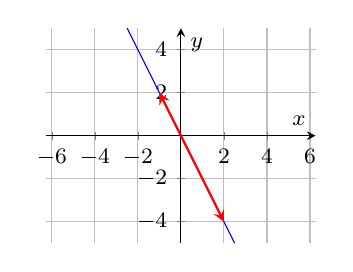
\begin{tikzpicture}[]
\begin{axis}[footnotesize,font=\footnotesize
    , axis equal, axis lines=middle,
    , xlabel={$x$},ylabel={$y$},  grid, domain=-2.5:2.5
    ]
    \addplot[blue]{-2*x} ;
    \addplot[red,quiver={u=-1,v=2},-stealth,thick] coordinates {(0,0)};
    \addplot[red,quiver={u=2,v=-4},-stealth,thick] coordinates {(0,0)};
\end{axis}
\end{tikzpicture}
}

\item  In 3D, \(\Span\{(-1,2,0),(0,2,1)\}\) is the set of all linear combinations \(s(-1,2,0)+t(0,2,1)\) which here is a parametric form of the plane illustrated below (Definition~\ref{def:parpla}).  
The plane passes through the origin~\ov, obtained when \(s=t=0\)\,.
%\marginpar{%
\begin{center}
\foreach \q in {37,40} {\begin{tikzpicture}
\begin{axis}[footnotesize,view={\q}{30}
    , grid, domain=-1:1 ]
    \addplot3[surf,shader=interp,blue,opacity=0.4,samples=2,y domain=-0.5:4] {x+y/2};
    \addplot3[red,quiver={u=-1,v=2,w=0},-stealth,thick] coordinates {(0,0,0)};
    \addplot3[red,quiver={u=0,v=2,w=1},-stealth,thick] coordinates {(0,0,0)};
\end{axis}
\end{tikzpicture}}
\end{center}
One could also check that the vector~\((2,1,-2)\) is orthogonal to these two vectors, hence is a normal to the plane, and so the plane may be also expressed as \(2x+y-2z=0\)\,.

\item For the complete set of \(n\)~standard unit vectors in~\(\RR^n\), \(\Span\{\hlist\ev n\}=\RR^n\).
This is because any vector \(\xv=(\hlist xn)\) in~\(\RR^n\) may be written as the linear combination \(\xv=x_1\ev_1+x_2\ev_2+\cdots+x_n\ev_n\) and hence is in \(\Span\{\hlist\ev n\}\).


\item The homogeneous system (Definition~\ref{def:homosys}) of linear equations from Example~\ref{eg:homosysiv} has solutions \(\xv=(-2s-\frac{15}7t,s,\frac97t,t) =(-2,1,0,0)s+(-\frac{15}7,0,\frac97,1)t\) for arbitrary \(s\) and~\(t\).
That is, the set of solutions is \(\Span\{(-2,1,0,0),\linebreak[1](-\frac{15}7,0,\frac97,1)\}\), a subset of~\(\RR^4\).

Generally, the set of solutions to a homogeneous system is the span of some set.

\item However, the set of solutions to a non-homogeneous system is generally not equal to the span of some set.  
For example, the solutions to Example~\ref{eg:gjeb} are all of the form \((u,v,w)=(-\frac34-\frac14t,\frac12+\frac32t,t) 
=(-\frac34,\frac12,0)+t(-\frac14,\frac32,1)\) for arbitrary~\(t\).
True, each of these solutions is a linear combination of vectors \((-\frac34,\frac12,0)\) and \((-\frac14,\frac32,1)\). 
But the multiple of \((-\frac34,\frac12,0)\) is always fixed, whereas the span invokes \emph{all} multiples.
Consequently, all the possible solutions cannot be the same as the span of some vectors.


\end{enumerate}
\end{example}



\begin{example} \label{eg:}
Describe in other words \(\Span\{\iv,\kv\}\) in~\(\RR^3\).

\begin{solution} 
All vectors in \(\Span\{\iv,\kv\}\) are of the form
\(c_1\iv+c_2\kv
=c_1(1,0,0)+c_2(0,0,1)
=(c_1,0,c_2)\).
Hence the span is all vectors with second component zero---the plane \(y=0\) in \((x,y,z)\) coordinates.
\end{solution}
\end{example}



\begin{example} \label{eg:}
Find a set~\(S\) such that \(\Span S=\{(3b,a+b,-2a-4b): a,b\text{ scalars}\}\).
Similarly, find a set~\(T\) such that \(\Span T=\{(-a-2b-2,-b+1, -3b-1): a,b\text{ scalars}\}\).
\begin{solution} 
Because vectors \((3b,a+b,-2a-4b)=a(0,1,-2)+b(3,1,-4)\) for all scalars~\(a\) and~\(b\),  a suitable set is \(S=\{(0,1,-2),\linebreak[1] (3,1,-4)\}\). 

Second, vectors \((-a-2b-2,-b+1, 3b-1)=a(-1,0,0)+b(-2,-1,3)+(-2,1,-1)\) which are linear combinations for all \(a\) and~\(b\). 
However, the vectors cannot form a span due to the constant vector \((-2,1,-1)\) because a span requires \emph{all} linear combinations of its component vectors.
The given set cannot be expressed as a span. 
\end{solution}
\end{example}





Geometrically, the span of a set of vectors is always all vectors lying in either a line, a plane, or  a higher dimensional hyper-plane, that passes \emph{through the origin} (discussed further by section~\ref{sec:sbd}).


\begin{comment}
Do not introduce ``Linear Independence'' yet as orthogonality is more important in applications---leave it until Chapter~\ref{ch:gee}.  
Instead soon introduce the more commonly invoked concept of orthonormal vectors.
\end{comment}




%\section{Applications}
%
%
%\begin{comment}
%Need to choose application(s) from: 
%Allocation of resources; 
%Balancing chemical equations; 
%Network analysis;
%Electrical Networks;
%Linear economic models;
%Finite linear games.
%Maybe better to interleave, or to use to revise material previously met. 
%\end{comment}



\subsection{Exercises}



\begin{exercise} \label{ex:} 
For each of the following, express vectors~\av\ and~\bv\ as a \idx{linear combination} of vectors~\(\vv_1\) and~\(\vv_2\).
Estimate the coefficients roughly (to say~10\%).
\newcommand{\pvec}[3]{%
    \pgfmathparse{(#1)*0.7+(#2)*0.1}\let\h\pgfmathresult
    \pgfmathparse{(#2)*0.7-(#1)*0.1}\let\v\pgfmathresult
    \edef\mytmp{\noexpand
    \addplot[\vcol,thick,quiver={u=#1,v=#2},-stealth] coordinates {(0,0)};
    \noexpand\node[] at (axis cs:\h,\v) {#3};
    }\mytmp
    }
\newcommand{\mytemp}[8]{\item
\begin{tikzpicture} 
\begin{axis}[footnotesize,font=\footnotesize
    ,axis equal, axis lines=none ] 
    \addplot[] coordinates {(0,0)};
    \def\vcol{red}
    \pvec{#1}{#2}{$\noexpand\vv_1$};
    \pvec{#3}{#4}{$\noexpand\vv_2$};
    \def\vcol{blue}
    \pvec{#5*#1+#6*#3}{#5*#2+#6*#4}{$\noexpand\av$};
    \pvec{#7*#1+#8*#3}{#7*#2+#8*#4}{$\noexpand\bv$};
\end{axis}
\end{tikzpicture}
\answer{$\noexpand\av=#5 \noexpand\vv_1 #6 \noexpand\vv_2$, 
$\noexpand\bv=#7 \noexpand\vv_1 #8 \noexpand\vv_2$}
}

\begin{parts}

\mytemp{-1.0}{0.5}{0}{0.9}{1}{+1}{1.5}{-0.5}

\mytemp{-3.3}{ 2.9}{-0.5}{-2.4}{-1}{+1.5}{ 1}{+3}

\mytemp{-0.9}{-1.3}{-0.5}{ 1.6}{-0.8}{+0}{ 2}{-0.5}

\mytemp{1.8}{-0.1}{-0.2}{-1.9}{ 0.3}{-1.7}{-1.4}{+3.3}

\mytemp{1.5}{-0.8}{-0.7}{-1.0}{ 0.9}{+1.1}{ 3.6}{-1.0}

\mytemp{-1.2}{ 0.3}{-0.4}{-0.5}{ 2.3}{-2.6}{-1.4}{-0.4}

\mytemp{0.4}{-1.3}{-2.9}{-1.7}{-2.6}{+0.9}{1.0}{+0.9}

\mytemp{-0.4}{-1.9}{1.4}{0.5}{-1.8}{+1.5}{-1.5}{-0.6}

\end{parts}
\end{exercise}





\begin{exercise} \label{ex:} 
For each of the following lines in 2D, write down a \idx{parametric equation} of the line as a \idx{linear combination} of two vectors, one of which is multiplied by the parameter.
\newcommand{\mytemp}[4]{\item
\begin{tikzpicture} 
\begin{axis}[footnotesize,font=\footnotesize
    ,axis equal, axis lines=middle, grid, domain=-4.5:4.5 ] 
    \addplot[blue,thick] {#2+(x-(#1))*(#4)/(#3)};
\end{axis}
\end{tikzpicture}
\answer{e.g.\ $(#1,#2)+t(#3,#4)$}
}

\begin{parts}
\mytemp{-0.5}{-2}{-1.5}{0}

\mytemp{0}{3.5}{-2.5}{2}

\mytemp{0}{-0.5}{-1}{0}

\mytemp{-1.5}{0.5}{1}{-1.5}

\mytemp{-1.5}{-3}{-1}{-1}

\mytemp{0.5}{1}{0.5}{1}
\end{parts}
\end{exercise}




\begin{exercise} \label{ex:syslc} 
Write each of the following systems of linear equations as one vector equation involving a \idx{linear combination} of vectors.
\begin{parts}
\item\label{ex:syslci} \(\begin{array}{l}
-2x+y-2z=-2\\
-4x+2y-z=2
\end{array}\)
\answer{\(\begin{bmatrix} -2\\-4 \end{bmatrix}x
+\begin{bmatrix} 1\\2 \end{bmatrix}y
+\begin{bmatrix} -2\\-1 \end{bmatrix}z=
\begin{bmatrix} -2\\2 \end{bmatrix}\)}

\item\label{ex:syslcii} \(\begin{array}{l}
-3x+2y-3z=0\\
y-z=0\\
x-3y=0
\end{array}\)
\answer{\(\begin{bmatrix} -3\\0\\1 \end{bmatrix}x
+\begin{bmatrix} 2\\1\\-3 \end{bmatrix}y
+\begin{bmatrix} -3\\1\\0 \end{bmatrix}z=
\begin{bmatrix} 0\\0\\0 \end{bmatrix}\)}

\item\label{ex:syslciii} \(\begin{array}{l}
x_1+   3x_2+   x_3  -2x_4=   2\\
   2x_1+   x_2+   4x_3  -2x_4=  -1\\
  -x_1+   2x_2  -2x_3  -x_4=   3
\end{array}\)
\answer{\(\begin{bmatrix} 1\\2\\-1 \end{bmatrix}x_1
+\begin{bmatrix} 3\\1\\2 \end{bmatrix}x_2
+\begin{bmatrix} 1\\4\\-2 \end{bmatrix}x_3
+\begin{bmatrix} -2\\-2\\-1 \end{bmatrix}x_4=
\begin{bmatrix} 2\\-1\\3 \end{bmatrix}\)}

\item\label{ex:syslciv} \(\begin{array}{l}
  -2p  -2q=  -1\\
      q=   2\\
   3p  -q=  1\\
\end{array}\)
\answer{\(\begin{bmatrix} -2\\0\\3 \end{bmatrix}p
+\begin{bmatrix} -2\\1\\-1 \end{bmatrix}q
=\begin{bmatrix} -1\\2\\1 \end{bmatrix}\)}

\end{parts}
\end{exercise}


\begin{exercise} \label{ex:} 
For each of the cases in Exercise~\ref{ex:syslc}, by attempting to solve the system, determine if the right-hand side vector is in the span of the vectors on the left-hand side.
\answer{\ref{ex:syslci}, yes,  e.g.\ \((x,y,z)=(0,2,2)\);
\ref{ex:syslcii}, yes,  e.g.\ \((x,y,z)=(0,0,0)\);
\ref{ex:syslciii}, yes,  e.g.\ \(\xv=(-1,1,0,0)\);
\ref{ex:syslciv}, no, as there is no solution for \(p\) and~\(q\).}
%\begin{answer}
%\begin{parts}
%\item  yes, e.g.\ \((x,y,z)=(0,2,2)\);
%\item yes,  e.g.\ \((x,y,z)=(0,0,0)\);
%\item yes,  e.g.\ \(\xv=(-1,1,0,0)\);
%\item no, as there is no solution for \(p\) and~\(q\).
%\end{parts}
%\end{answer}
\end{exercise}




\begin{exercise} \label{ex:} 
For each of the following sets, write the set as a span, if possible.
Give reasons.
\begin{enumerate}
\item \(\{(p-4q,p+2q,p+2q): p,q\text{ scalars}\}\)
\answer{e.g.\ \(\Span\{(1,1,1), (-4,2,2)\}\)}

\item \(\{(-p+2r,2p-2q,p+2q+r,-q-3r): p,q,r\text{ scalars}\}\)
\answer{e.g.\ \(\Span\{(-1,2,1,0), (0,-2,2,-1), (2,0,1,-3)\}\)}

\item The line \(y=2x+1\) in \(\RR^2\).
\answer{Not a span.}

\item The line \(x=y=z\) in \(\RR^3\).
\answer{e.g.\ \(\Span\{(1,1,1)\}\).}

\item The set of vectors~\(\xv\) in~\(\RR^4\) with component \(x_3=0\)\,.
\answer{e.g.\ \(\Span\{\ev_1,\ev_2,\ev_4\}\).}
\end{enumerate}
\end{exercise}







\begin{exercise} \label{ex:} 
Show the following identities hold for any given vectors \uv,\vv\ and~\wv:
\begin{enumerate}
\item \(\Span\{\uv,\vv\}=\Span\{\uv-\vv,\uv+\vv\}\);
\item \(\Span\{\uv,\vv,\wv\}=\Span\{\uv,\uv-\vv,\uv+\vv+\wv\}\).
\end{enumerate}
\end{exercise}








\begin{exercise} \label{ex:} 
Suppose \hlist\uv s\ are any \(s\)~vectors in~\(\RR^n\).
Let set \(R=\{\hlist\uv r\}\) for some \(r<s\), and set \(S=\{\hlist\uv r,\uv_{r+1},\ldots,\uv_s\}\).
\begin{enumerate}
\item Prove that \(\Span R\subseteq\Span S\)\,.
\item Hence deduce that if \(\Span R=\RR^n\), then \(\Span S=\RR^n\).
\end{enumerate}
\end{exercise}




\begin{exercise} \label{ex:} 
Suppose \hlist\uv r\ and \hlist\vv s\ are all vectors in~\(\RR^n\).
\begin{enumerate}
\item Prove that if every vector~\(\uv_j\) is a linear combination of \hlist\vv s, then \(\Span\{\hlist\uv r\}\subseteq\Span\{\hlist\vv s\}\).
\item  Prove that if, additionally, every vector~\(\vv_j\) is a linear combination of \hlist\uv r, then \(\Span\{\hlist\uv r\}=\Span\{\hlist\vv s\}\).
\end{enumerate}
\end{exercise}





\begin{exercise} \label{ex:} 
Let \(S=\{\hlist\vv s\}\) be a set of vectors in~\(\RR^n\) such that vector~\(\vv_1\) is a linear combination of \hlist[2]\vv s\,.  
Prove that \(\Span S=\Span\{\hlist[2]\vv s\}\).
\end{exercise}







\begin{comment}%{ED498555.pdf}
why, what caused X?
how did X occur?
what-if? what-if-not?
how does X compare with Y?
what is the evidence for X?
why is X important?
\end{comment}



